\documentclass[border=8pt]{standalone}
\usepackage[T1]{fontenc}\usepackage{helvet}\renewcommand{\familydefault}{\sfdefault}
\usepackage{tikz}\usetikzlibrary{arrows.meta, positioning, calc, backgrounds}
\definecolor{ink}{HTML}{1a1916}
\definecolor{inktwo}{HTML}{3a3a35}
\definecolor{inkthree}{HTML}{6a6862}
\definecolor{rule}{HTML}{b8b09a}
\definecolor{amber}{HTML}{a8730a}
\definecolor{red}{HTML}{c8261a}
\definecolor{paper}{HTML}{f0eee5}
\definecolor{slab}{HTML}{d8d4c6}
\tikzset{
  >={Stealth[length=2.2mm]},
  wire/.style={line width=0.8pt, ink},
  modwire/.style={line width=0.6pt, dashed, ink},
  tastewire/.style={line width=0.6pt, dashed, amber},
  gatewire/.style={line width=0.6pt, dotted, ink},
  block/.style={rectangle, draw=ink, line width=0.9pt, fill=slab, minimum width=3.0cm, minimum height=1.9cm, inner sep=0pt},
  perf/.style={rectangle, draw=ink, line width=0.7pt, minimum width=3.0cm, minimum height=0.7cm, inner sep=2pt, font=\footnotesize, text=ink},
  title/.style={font=\scriptsize\bfseries, text=ink, anchor=north, inner sep=2pt},
  jack/.style={circle, draw=ink, fill=paper, line width=0.5pt, minimum size=3.2pt, inner sep=0pt},
  plabel/.style={font=\tiny, text=inktwo, anchor=west, inner sep=1pt},
  olabel/.style={font=\tiny, text=inktwo, anchor=east, inner sep=1pt},
  settings/.style={font=\scriptsize, text=ink, align=left, anchor=north west, inner sep=1pt, text width=2.9cm},
}
\begin{document}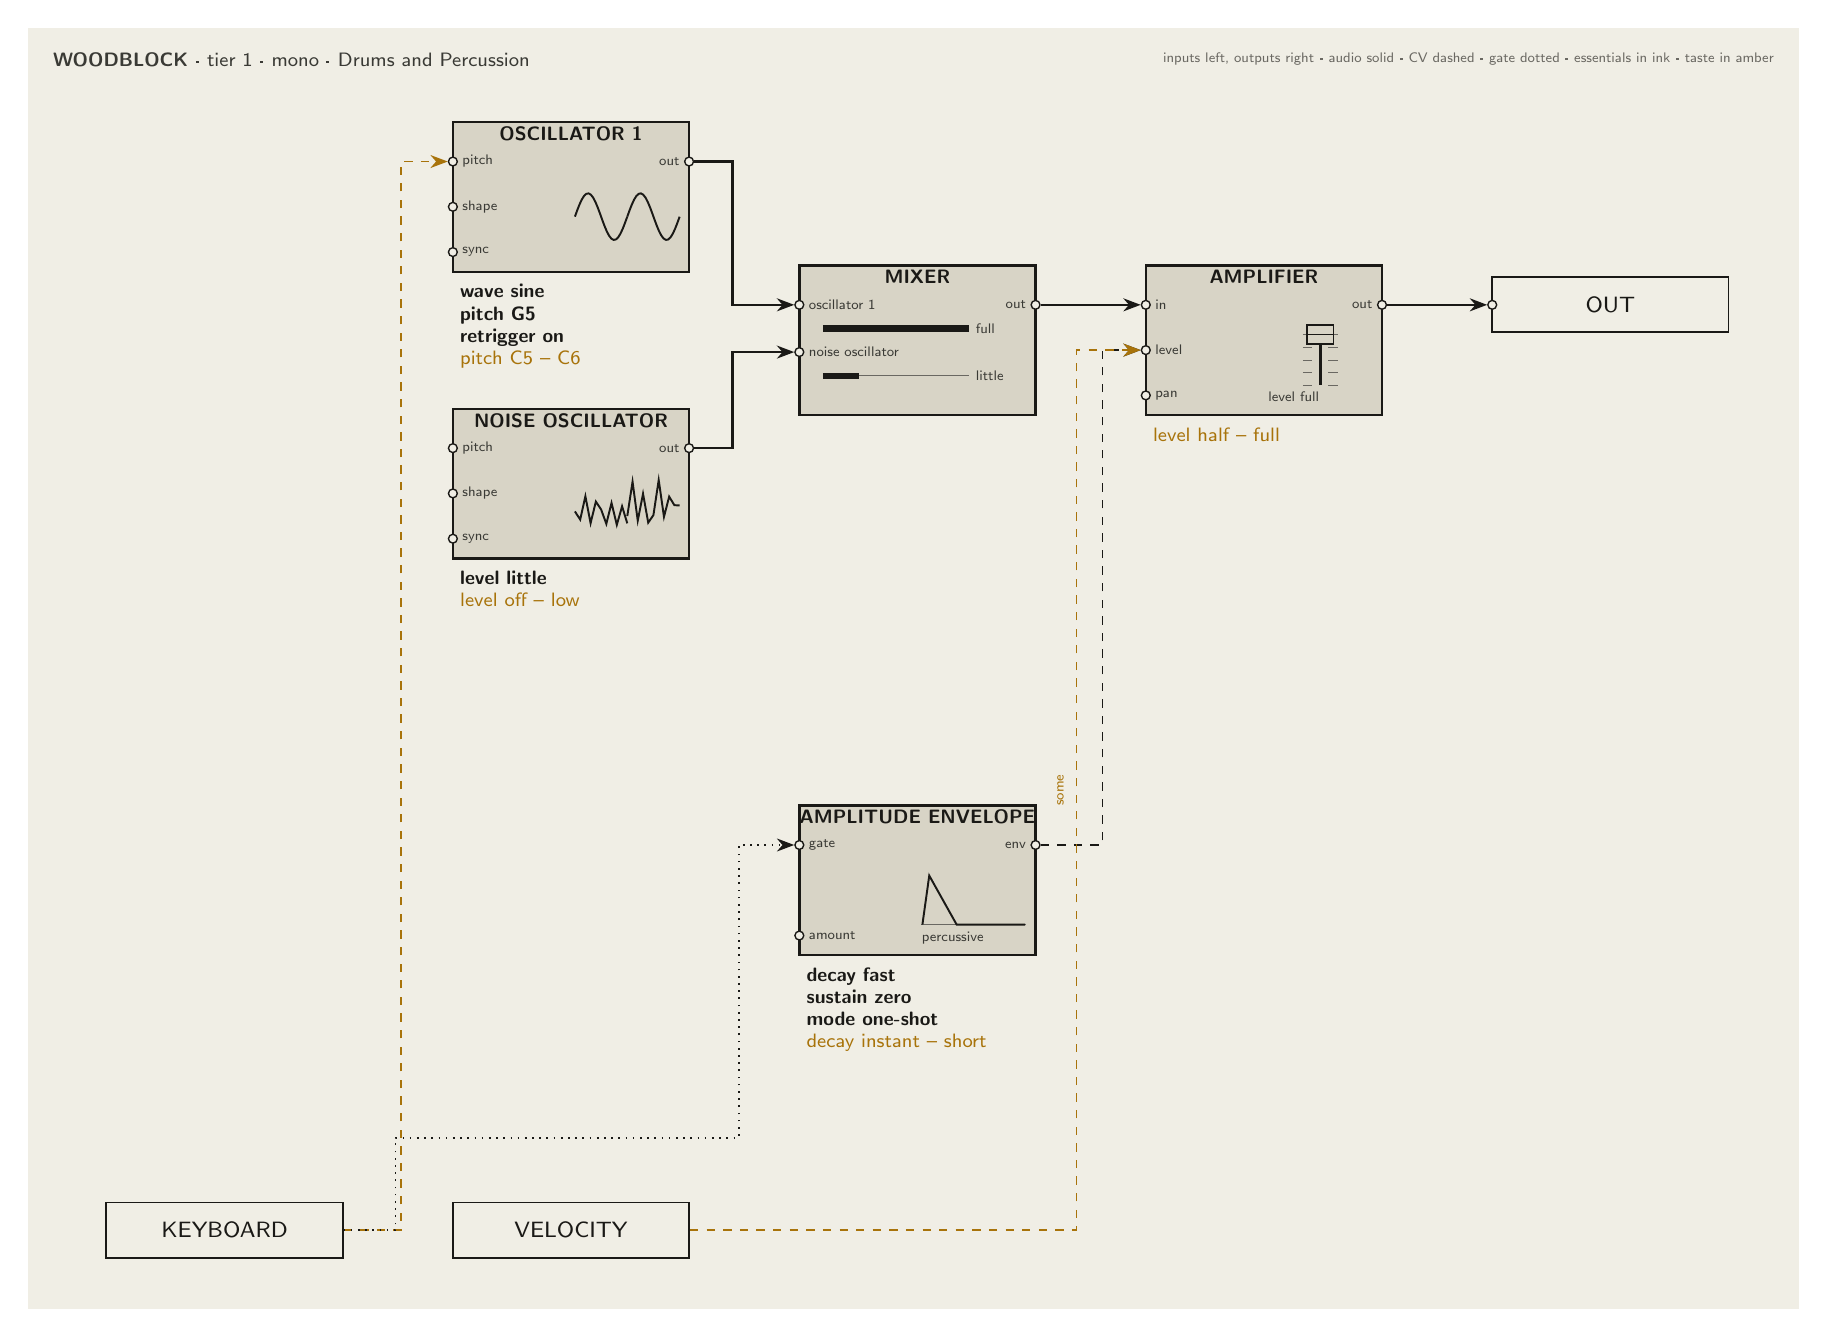
\begin{tikzpicture}
\begin{scope}[on background layer]\fill[paper] (-2.5,-12.299999999999999) rectangle (20.0,3.9699999999999998);\end{scope}
\node[block, minimum height=1.9cm] (osc1) at (4.4,1.8199999999999998) {};
\node[title] at (osc1.north) {OSCILLATOR 1};
\node[jack] (osc1-pitch) at (2.9000000000000004,2.2699999999999996) {};
\node[plabel] at (2.9800000000000004,2.2699999999999996) {pitch};
\node[jack] (osc1-shape) at (2.9000000000000004,1.6949999999999996) {};
\node[plabel] at (2.9800000000000004,1.6949999999999996) {shape};
\node[jack] (osc1-sync) at (2.9000000000000004,1.1199999999999997) {};
\node[plabel] at (2.9800000000000004,1.1199999999999997) {sync};
\node[jack] (osc1-out) at (5.9,2.2699999999999996) {};
\node[olabel] at (5.82,2.2699999999999996) {out};
\begin{scope}
\draw[ink, line width=0.7pt] plot[domain=0.000:0.500, samples=24, variable=\u] ({4.450+\u*1.330},{1.200+(0.740)*(0.5+0.4*sin(360*(\u*2))+0.0)});
\draw[ink, line width=0.7pt] plot[domain=0.500:1.000, samples=24, variable=\u] ({4.450+\u*1.330},{1.200+(0.740)*(0.5+0.4*sin(360*(\u*2))+0.0)});
\end{scope}
\node[settings] at (2.95,0.7499999999999999) {\textbf{wave sine} \\ \textbf{pitch G5} \\ \textbf{retrigger on} \\ \textcolor{amber}{pitch C5 -- C6}};
\node[block, minimum height=1.9cm] (noise) at (4.4,-1.8199999999999998) {};
\node[title] at (noise.north) {NOISE OSCILLATOR};
\node[jack] (noise-pitch) at (2.9000000000000004,-1.3699999999999999) {};
\node[plabel] at (2.9800000000000004,-1.3699999999999999) {pitch};
\node[jack] (noise-shape) at (2.9000000000000004,-1.9449999999999998) {};
\node[plabel] at (2.9800000000000004,-1.9449999999999998) {shape};
\node[jack] (noise-sync) at (2.9000000000000004,-2.5199999999999996) {};
\node[plabel] at (2.9800000000000004,-2.5199999999999996) {sync};
\node[jack] (noise-out) at (5.9,-1.3699999999999999) {};
\node[olabel] at (5.82,-1.3699999999999999) {out};
\begin{scope}
\draw[ink, line width=0.7pt] (4.450,-2.174) -- (4.517,-2.277) -- (4.583,-1.981) -- (4.649,-2.323) -- (4.716,-2.049) -- (4.783,-2.150) -- (4.849,-2.332) -- (4.915,-2.066) -- (4.982,-2.344) -- (5.049,-2.109) -- (5.115,-2.325);
\draw[ink, line width=0.7pt] (5.115,-2.232) -- (5.182,-1.796) -- (5.248,-2.291) -- (5.315,-1.949) -- (5.381,-2.316) -- (5.447,-2.220) -- (5.514,-1.775) -- (5.581,-2.242) -- (5.647,-1.986) -- (5.713,-2.094) -- (5.780,-2.098);
\end{scope}
\node[settings] at (2.95,-2.8899999999999997) {\textbf{level little} \\ \textcolor{amber}{level off -- low}};
\node[block, minimum height=1.9cm] (mix) at (8.8,0.0) {};
\node[title] at (mix.north) {MIXER};
\node[jack] (mix-osc1) at (7.300000000000001,0.44999999999999996) {};
\node[plabel] at (7.380000000000001,0.44999999999999996) {oscillator 1};
\draw[inkthree, line width=0.3pt] (7.600,0.150) -- (9.450,0.150);
\draw[ink, line width=2.2pt] (7.600,0.150) -- (9.450,0.150);
\node[font=\tiny, text=inktwo, anchor=west, inner sep=1pt] at (9.500,0.150) {full};
\node[jack] (mix-noise) at (7.300000000000001,-0.15000000000000002) {};
\node[plabel] at (7.380000000000001,-0.15000000000000002) {noise oscillator};
\draw[inkthree, line width=0.3pt] (7.600,-0.450) -- (9.450,-0.450);
\draw[ink, line width=2.2pt] (7.600,-0.450) -- (8.062,-0.450);
\node[font=\tiny, text=inktwo, anchor=west, inner sep=1pt] at (9.500,-0.450) {little};
\node[jack] (mix-out) at (10.3,0.44999999999999996) {};
\node[olabel] at (10.22,0.44999999999999996) {out};
\node[block, minimum height=1.9cm] (amp) at (13.200000000000001,0.0) {};
\node[title] at (amp.north) {AMPLIFIER};
\node[jack] (amp-in) at (11.700000000000001,0.44999999999999996) {};
\node[plabel] at (11.780000000000001,0.44999999999999996) {in};
\node[jack] (amp-level) at (11.700000000000001,-0.125) {};
\node[plabel] at (11.780000000000001,-0.125) {level};
\node[jack] (amp-pan) at (11.700000000000001,-0.7) {};
\node[plabel] at (11.780000000000001,-0.7) {pan};
\node[jack] (amp-out) at (14.700000000000001,0.44999999999999996) {};
\node[olabel] at (14.620000000000001,0.44999999999999996) {out};
\begin{scope}
\draw[ink, line width=1.2pt] (13.915,-0.570) -- (13.915,0.070);
\draw[inkthree, line width=0.3pt] (13.695,-0.570) -- (13.815,-0.570) (14.015,-0.570) -- (14.135,-0.570);
\draw[inkthree, line width=0.3pt] (13.695,-0.410) -- (13.815,-0.410) (14.015,-0.410) -- (14.135,-0.410);
\draw[inkthree, line width=0.3pt] (13.695,-0.250) -- (13.815,-0.250) (14.015,-0.250) -- (14.135,-0.250);
\draw[inkthree, line width=0.3pt] (13.695,-0.090) -- (13.815,-0.090) (14.015,-0.090) -- (14.135,-0.090);
\draw[inkthree, line width=0.3pt] (13.695,0.070) -- (13.815,0.070) (14.015,0.070) -- (14.135,0.070);
\fill[slab, draw=ink, line width=0.6pt] (13.745,-0.050) rectangle (14.085,0.190);
\draw[ink, line width=0.5pt] (13.745,0.070) -- (14.085,0.070);
\node[font=\tiny, text=inktwo, anchor=north west, inner sep=0pt] at (13.250,-0.650) {level full};
\end{scope}
\node[settings] at (11.750000000000002,-1.0699999999999998) {\textcolor{amber}{level half -- full}};
\node[block, minimum height=1.9cm] (aenv) at (8.8,-6.86) {};
\node[title] at (aenv.north) {AMPLITUDE ENVELOPE};
\node[jack] (aenv-gate) at (7.300000000000001,-6.41) {};
\node[plabel] at (7.380000000000001,-6.41) {gate};
\node[jack] (aenv-amount) at (7.300000000000001,-7.5600000000000005) {};
\node[plabel] at (7.380000000000001,-7.5600000000000005) {amount};
\node[jack] (aenv-out) at (10.3,-6.41) {};
\node[olabel] at (10.22,-6.41) {env};
\begin{scope}
\draw[inkthree, line width=0.3pt] (8.850,-7.421) -- (10.180,-7.421);
\draw[ink, line width=0.7pt] (8.863,-7.421) -- (8.950,-6.799) -- (9.298,-7.421) -- (9.298,-7.421) -- (10.167,-7.421);
\node[font=\tiny, text=inktwo, anchor=north west, inner sep=0pt] at (8.850,-7.510) {percussive};
\end{scope}
\node[settings] at (7.3500000000000005,-7.930000000000001) {\textbf{decay fast} \\ \textbf{sustain zero} \\ \textbf{mode one-shot} \\ \textcolor{amber}{decay instant -- short}};
\node[perf] (key) at (0.0,-11.299999999999999) {KEYBOARD};
\node[perf] (vel) at (4.4,-11.299999999999999) {VELOCITY};
\node[perf, fill=paper] (out) at (17.6,0.44999999999999996) {OUT}; \node[jack] (out-in) at (16.1,0.44999999999999996) {};
\draw[wire,->] (osc1-out) -- (6.45,2.2699999999999996) |- (mix-osc1);
\draw[wire,->] (noise-out) -- (6.45,-1.3699999999999999) |- (mix-noise);
\draw[wire,->] (mix-out) -- (amp-in);
\draw[wire,->] (amp-out) -- (out-in);
\draw[modwire,->] (aenv-out) -- (11.15,-6.41) -- (11.15,-0.125) -- (amp-level);
\draw[tastewire,->] (key.east) -- (2.2400000000000007,-11.299999999999999) -- (2.2400000000000007,2.2699999999999996) -- (osc1-pitch);
\draw[gatewire,->] (key.east) -- (2.17,-11.299999999999999) -- (2.17,-10.13) -- (6.530000000000001,-10.13) -- (6.530000000000001,-6.41) -- (aenv-gate);
\draw[tastewire,->] (vel.east) -- (10.82,-11.299999999999999) -- (10.82,-0.125) -- (amp-level);
\node[font=\tiny, text=amber, anchor=south, inner sep=1pt, rotate=90] at (10.700000000000001,-5.7124999999999995) {some};
\node[anchor=north west, font=\scriptsize, text=inktwo] at (-2.3,3.7699999999999996) {\textbf{WOODBLOCK} · tier 1 · mono · Drums and Percussion};
\node[anchor=north east, font=\tiny, text=inkthree] at (19.8,3.7699999999999996) {inputs left, outputs right · audio solid · CV dashed · gate dotted · essentials in ink · taste in amber};
\end{tikzpicture}\end{document}
